\documentclass[times]{article}

\usepackage{graphicx}
\usepackage{placeins}
\usepackage{float}
\usepackage[ruled,linesnumbered]{algorithm2e}
\usepackage[none]{hyphenat}
\usepackage{amsmath}
\newcommand{\thickhat}[1]{\mathbf{\hat{\text{$#1$}}}}
\usepackage[us]{datetime}
\usepackage[explicit]{titlesec}
\usepackage[margin=1.0in]{geometry}
\begin{document}
	\title{CS 6001 Applied Spatial and Temporal Data Analysis - Spring 2017 - Homework 4}
	\author{Dalton Cole}
	\date{\formatdate{3}{4}{2017}}
	\maketitle

	\section{Introduction}
		\paragraph{}
		The purpose of this assignment is to become familiar with recommender systems. In the video that Dr.Fu asked us to watch, User-based collaborative filtering and item-based collaborative filtering was discussed. This assignment gives us first hand experience at these two filtering methods. User-based collaborative filtering is done by finding the similarity between different users based on the items, in the video's case, Netflix shows watched. Item-based collaborative filtering is essentially the transpose of user-based. Similarity between items are used instead of between users. In most cases, this provides more reliable data. This is in part because, normally, there are fewer catalog items than there are users. This reduces the dimensionality of the data.
		\paragraph{}
		These two methods are variations of the kNN algorithm. The basic formula is:

		\begin{equation*}
		\hat{r}_{ui} = \frac{
		\sum\limits_{v \in N^k_i(u)} \text{sim}(u, v) \cdot r_{vi}}
		{\sum\limits_{v \in N^k_i(u)} \text{sim}(u, v)}
		\end{equation*}

		\paragraph{}
		Three more algorithms are used: SVD, PMF, and NMF. The SVD algorithm was popularized by Simon Funk, as discussed in the KNN tutorial video. It uses a prediction value:

		\begin{equation*}
		\hat{r}_{ui} = \mu + b_u + b_i + q_i^Tp_u
		\end{equation*}

		\paragraph{}
		The following regularized squared error should be minimized using stochastic gradient descent:

		\begin{equation*}
		\sum_{r_{ui} \in R_{train}} \left(r_{ui} - \hat{r}_{ui} \right)^2 +
		\lambda\left(b_i^2 + b_u^2 + ||q_i||^2 + ||p_u||^2\right)
		\end{equation*}

		\paragraph{}
		PMF is the unbiased version of SVD:

		\begin{equation*}
		\hat{r}_{ui} = q_i^Tp_u
		\end{equation*}

		\paragraph{}
		NMF is very similar to SVD as well. The difference between the two is that the user and item factors are kept positive in NMF.

		\paragraph{}
		MAE and RMSE are two matrices that are used to evaluate performance. Mean absolute error (MAE) can be seen in Figure \ref{equ:MAE}. Root-mean-square deviation (RMSD) can be found in Figure \ref{equ:RMSD}.


		\begin{figure}
			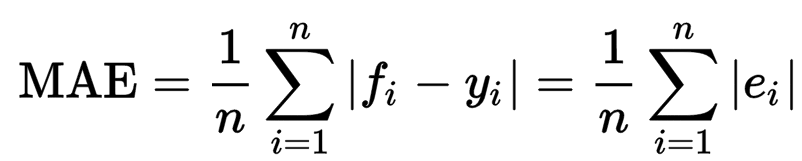
\includegraphics[width=\linewidth]{MAE}
			\caption{Mean Absolute Error Formula}
			\label{equ:MAE}
		\end{figure}

		\begin{figure}
			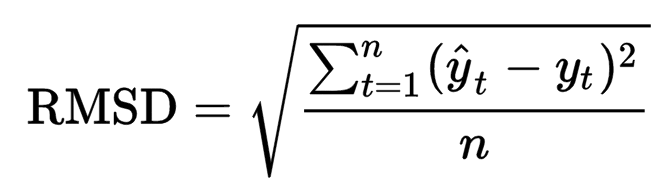
\includegraphics[width=\linewidth]{RMSD}
			\caption{Root-Mean-Square Deviation Formula}
			\label{equ:RMSD}
		\end{figure}

	\section{Experiment}
		\paragraph{}
		The code used for this segment can be found in \textit{HW4.py}. The data used in this experiment is located in \textit{restaurant\_ratings.txt}, which is a text file given by Dr.Fu for this assignment. The goal of this experiment is to see which algorithm performs best given this data set. Three-fold cross validation was used. To keep each fold consistent across each algorithm and across seperate tests, the random seed generator was seeded with the value \textit{0}. 

	\section{Results}
		\paragraph{}
		The results of this experiment can be seen in Figures \ref{fig:9}, \ref{fig:13}, \ref{fig:14}, and \ref{fig:means}. As can be seen in Figure \ref{fig:9}, SVD out performed the other methods. In this case, item-based collaborative filtering barely out performed user-based collaborative filtering. Figure \ref{fig:13} shows how important a similarity metric can be. Using the MSD similarity metric, item-based out performs user-based collaborative filtering. Using cosine or Pearson however gives user-based the edge. 

		\paragraph{}
		Figure \ref{fig:14} shows that when k = 25, 27, and 28, RMSE was as its minimal value for user-based collaborative filtering. This implies that looking at the mid 20s to higher 20s neighbors yields the best results for. When k = 43 gave item-based collaborative filtering its best RMSE value. Item-based out performed user-based when $k \geq 30$. When $k < 30$, user-based out performs item-based. 

		\begin{figure}
			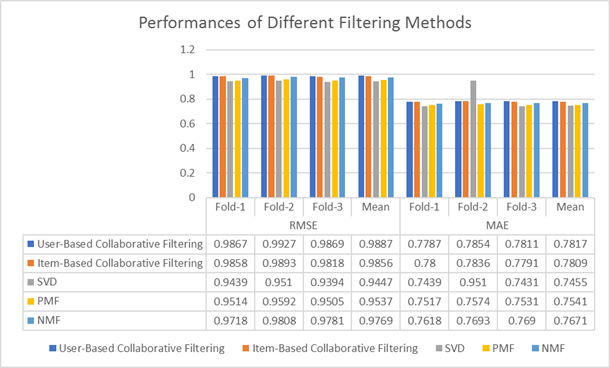
\includegraphics[width=\linewidth]{9.png}
			\caption{Performance of Different Filtering Methods}
			\label{fig:9}
		\end{figure}

		\begin{figure}
			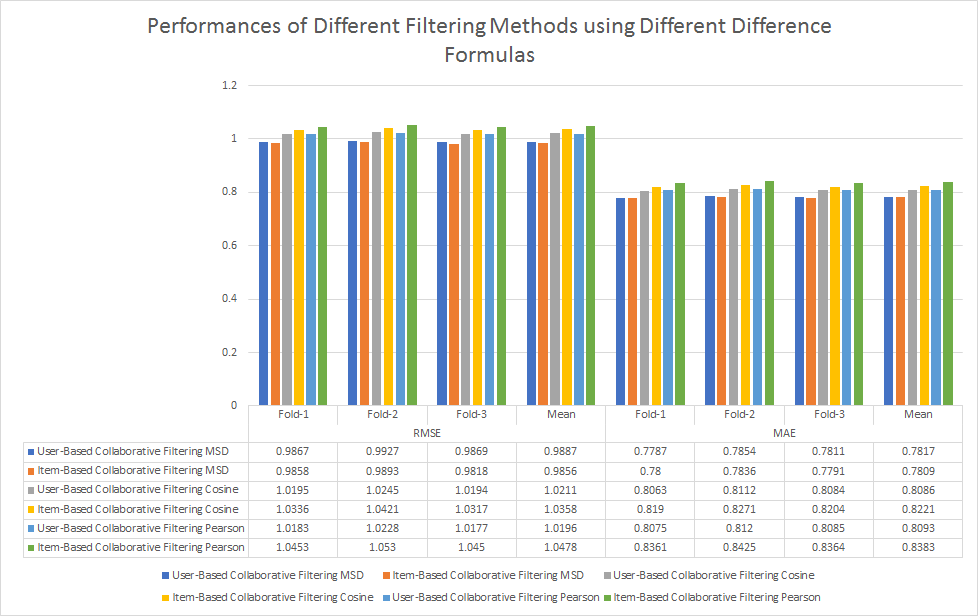
\includegraphics[width=\linewidth]{13.png}
			\caption{Performance of Different Filtering Methods using Different Difference Formulas}
			\label{fig:13}
		\end{figure}

		\begin{figure}
			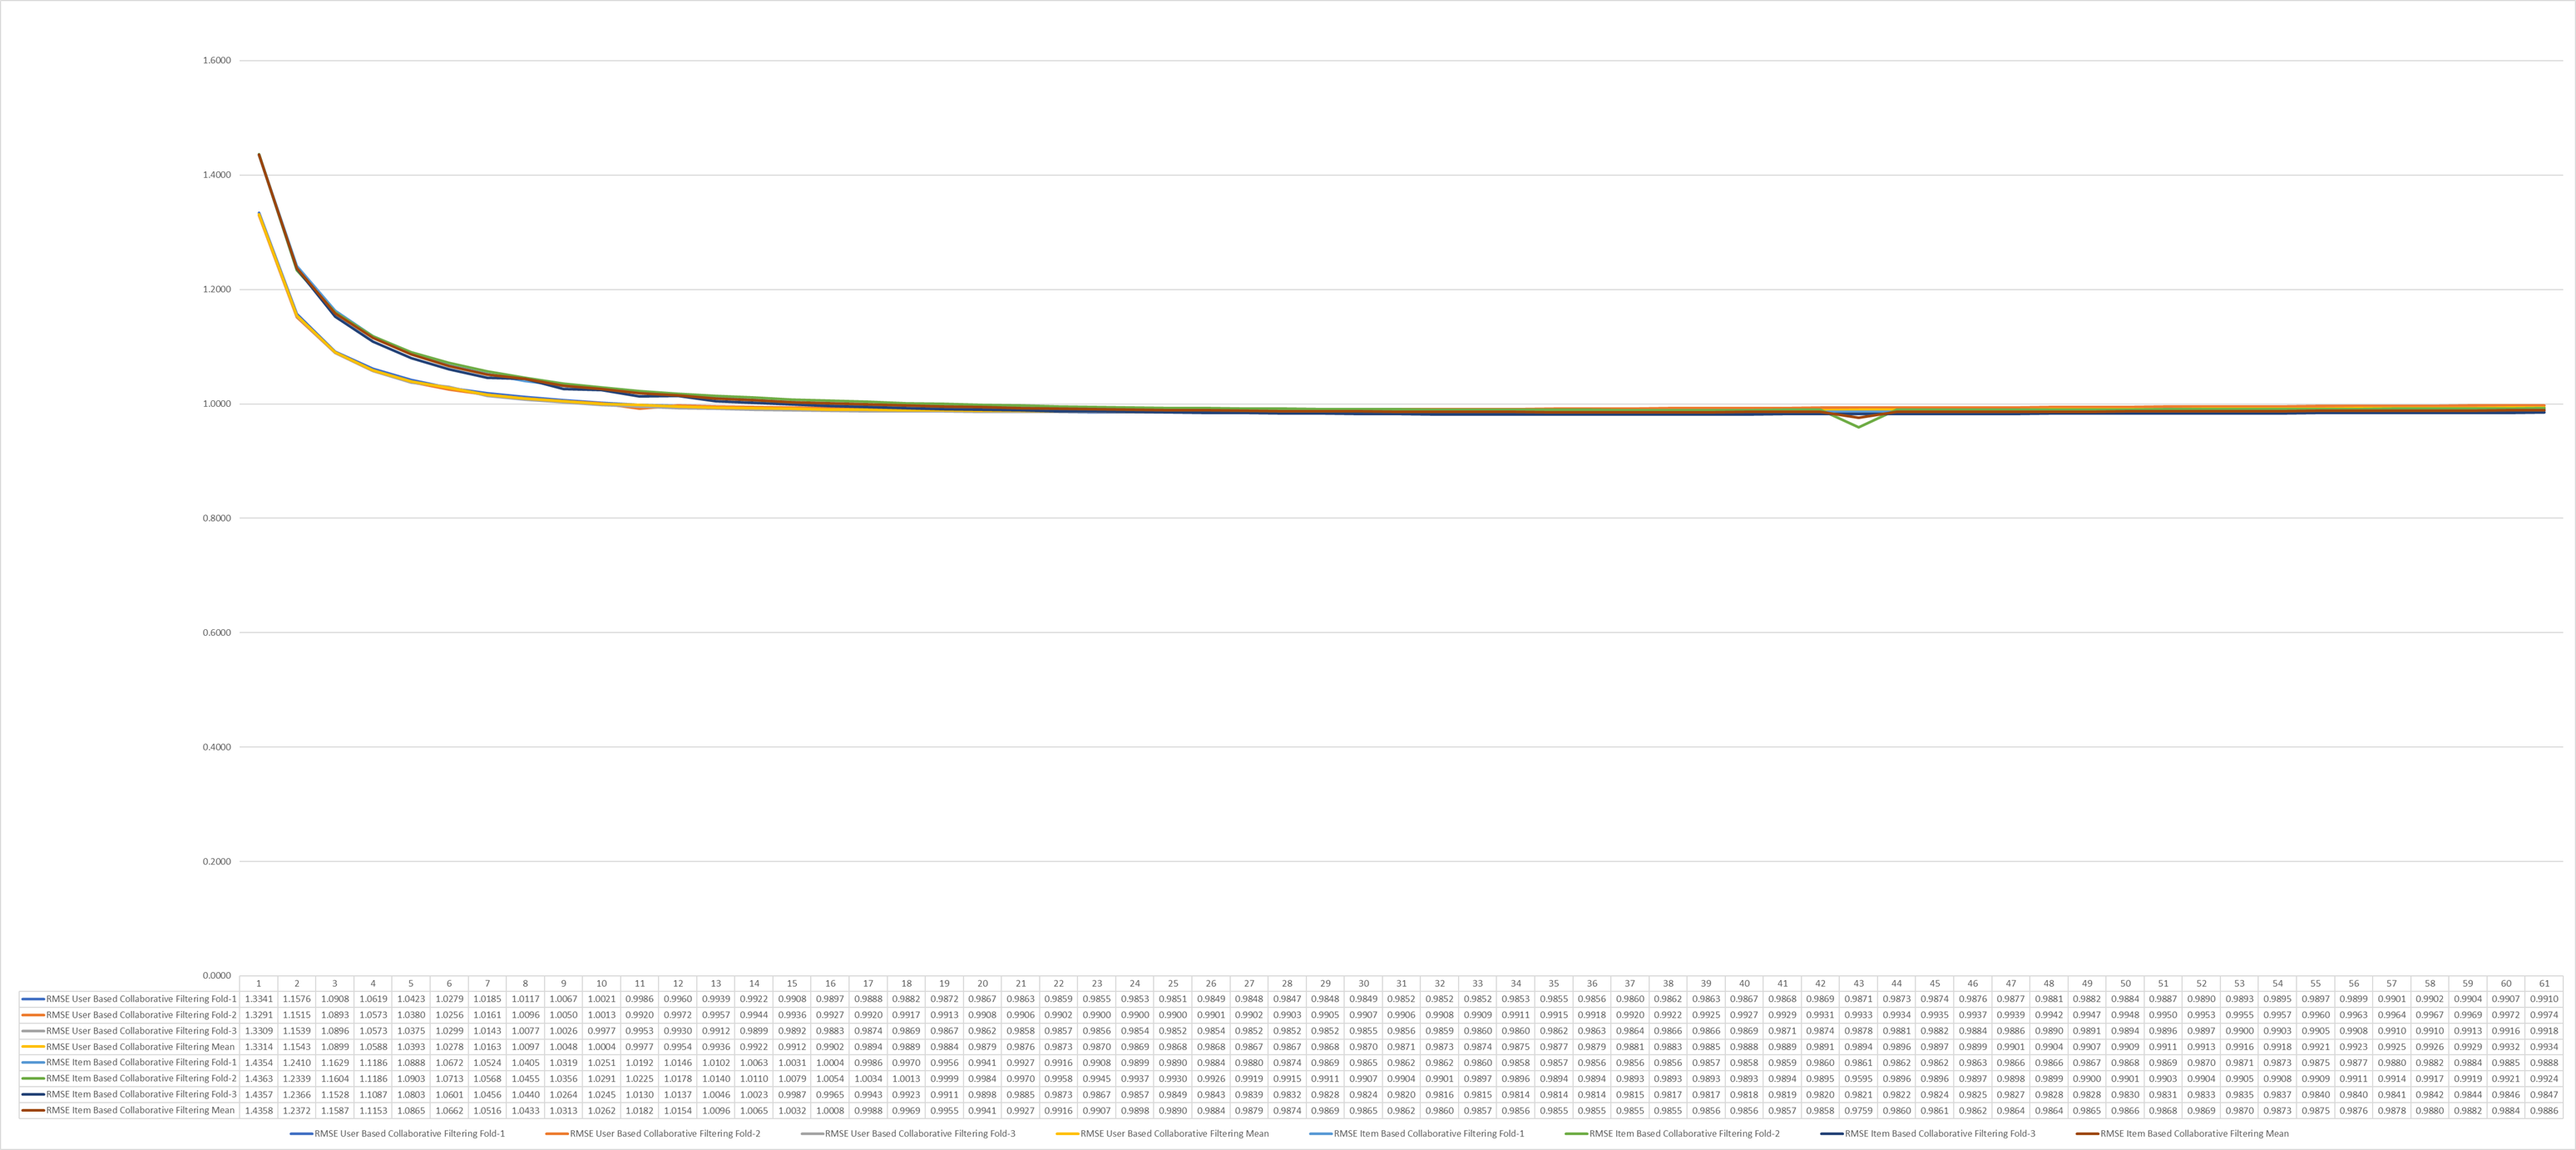
\includegraphics[width=\linewidth]{14.png}
			\caption{RMSE Filtering with each Fold and Mean of the Three Folds}
			\label{fig:14}
		\end{figure}

		\begin{figure}
			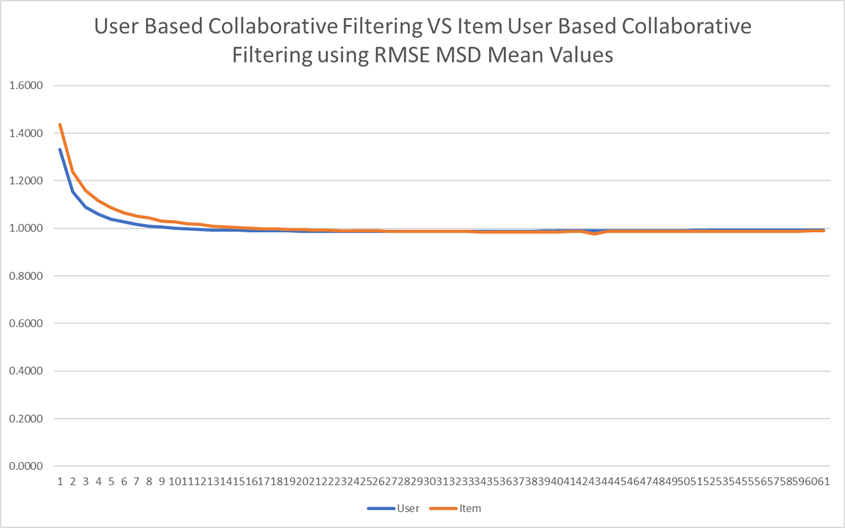
\includegraphics[width=\linewidth]{Means.png}
			\caption{User-Based Collaborative Filtering VS Item-Based Collaborative Filtering using RMSE MSD Mean Values}
			\label{fig:means}
		\end{figure}


	\section{Conclusion}
		\paragraph{}
		Different machine learning algorithms produce different results. Different error measuring formulas also produce different results. It is important to keep in mind both of these facts when selecting algorithms. It is important to be consistent with the error measurements. In this report, RMSE was primarily used to compare algorithms. It has been shown, that with the given data set, and with the given random folds, SVD is the best filtering algorithm out of the five in the experiment. Between user-based and item-based collaborative filtering, item-based generally out performed user-based. Since these two methods are variations of the kNN method, it is important to keep in mind the value of k. When k has a value less than 30, user-based collaborative filtering out performed item-based. This will vary depending on the data set, but the general trend that user-base will out perform item-based up until a certain threshold is expected.
		\paragraph{}
		Different similarity measurements matter highly as well. As shown in Figure \ref{fig:13}, item-based Pearson method performed the worst, however, out of the user-based methods, using the cosine similarity performed the worst. Different similarity measurements vary on different algorithms and data sets. 
		


\end{document}	






